\chapter{Exploratory Data Analysis- EDA}
\label{sec:exploratory}


In this chapter, we give a short review of methods for exploratory data analysis, a.k.a.\ \emph{descriptive statistics}.\marginnote{descriptive statistics}
Recall that our goal is an assumptions-free description of our data. 
EDA thus consist of computing interpretable summaries of the data, called \emph{summary statistics}, and visualizations. 


\section{Summary Statistics}
\label{sec:summary_statistics}

We now distinguish between summary statistics that apply to attributes, categorical by definition, and variables, continuous by definition. 


\subsection{Summarizing Categorical Data}

\subsubsection{Univariate}
Summarizing a vector of categorical data can naturally be done by tabulating it, i.e., computing the frequency and relative frequency of each category.
Clearly averages, medians, and the likes are incomputable, since categorical data has no ordering, nor does it admit simple operations such as summation.

\begin{extra}
Variability of categorical data can clearly not be measured by its variance, since it does not admit a summation operation.
It is, however, possible to define different measures of variability that do apply.
The \emph{entropy} is such an example.\marginnote{Entropy}
\end{extra}


\subsubsection{Bivariate}
Generalizing the univariate case to bivariate, or multivariate, one can keep tabulating. I.e., compute the frequency, and relative frequency, of combinations of categories.



\subsection{Summarizing  Continuous Data}
Continuous variables admit many more mathematical manipulations than categorical attributes. 


\subsubsection{Univariate}

We start by presenting the most natural summaries of the data. Without going into the formal definition, we refer to them as \emph{summary of location}.\marginnote{Location Summaries}
These include:

\begin{definition}[The Mean (Average)]
\begin{align}
	\bar{x}:= \frac{1}{n}\sum_{i=1}^{n} x_i
\end{align}
\end{definition}

\begin{definition}[The Median]
The median is the observation that is smaller than half of the sample and larger than half of the sample.
\end{definition}

\begin{definition}[$\alpha$-trimmed mean]
The $\alpha$-trimmed mean is the average of the observations left after ignoring the largest and the smallest $(100\alpha) \%$ of them.
\end{definition}
The \naive average is the $0$-trimmed mean, and the median is the $0.5$-trimmed mean.

From summaries of location, we move to summaries of \emph{scale}. \marginnote{Summary of Scale}

\begin{definition}[The Standard Deviation]
\begin{align}
	S^2(x):= \frac{1}{n-1} \sum_{i=1}^{n} (x_i-\bar{x})^2
\end{align}
\end{definition}

For the following, we require the definition of the sample quantiles, themselves \textbf{not} a scale summary.

\begin{definition}[$\alpha$ Quantile]
The $\alpha$-quantile of the sample is the observation that is larger than $(100\alpha)\%$, and smaller then  $(100(1-\alpha))\%$ of the sample. 
\end{definition}
The empirical maximum and minimum are then $x_{1.0}$ and $x_{0.0}$, respectively.


\begin{definition}[The Range]
\begin{align}
	Range(x):= \max_i\set{x_i}-\min_i\set{x_i}= x_{1.0}-x_{0.0}
\end{align}
\end{definition}

\begin{definition}[The Inter Quantile Range- IQR]
\label{def:iqr}
\begin{align}
	IQR(x):= x_{0.75}-x_{0.25}
\end{align}
\end{definition}



\begin{definition}[The Median Absolute Deviation- MAD]
\label{def:mad}
\begin{align}
	MAD(x):= \set{|x_i-x_{0.5}|}_{0.5}
\end{align}
\end{definition}
Note that the MAD may be sometimes scaled by some constant. Particularly in the \R function \texttt{mad()}. 


After summaries of scale, we move to summaries of \emph{skewness}, or \emph{asymmetry}.

\begin{definition}[Yule Skewness Measure]
[TODO: verify]
\begin{align}
	YULE(x):= \frac{(x_{0.75}+x_{0.25})-x_{0.5}}{2 IQR(x)}
\end{align}
\end{definition}

 


\subsubsection{Bivariate}
From univariate data $x$, we move to bivariate $x,y$.
Clearly we can apply univariate summaries component-wise. 
We want, however, to summarize the \emph{joint} behaviour of the data. 
For this purpose, we assume that data comes in pairs, implying that $x$ and $y$ are of same length.
The first measure, is naturally the celebrated (Pearson) correlation coefficient, that captures the level of linear association.


\begin{definition}[(Empirical) Covariance]
\begin{align}
	Cov(x,y):= \frac{\sum_{i=1}^{n} (x_i-\bar{x})(y_i-\bar{y})}{n-1}
\end{align}
\end{definition}



\begin{definition}[Pearson's Correlation Coefficient]
\begin{align}
	r(x,y):= \frac{(n-1) Cov(x,y)}{S(x) S(y)}
\end{align}
\end{definition}
We can dwell into the meaning and intuition underlying Pearson's correlation coefficient, but we will not. 
The curious reader is reffered to \cite{rodgers_thirteen_1988}.

The next measure of association captures a more general association.
\begin{definition}[Spearman's Correlation Coefficient]
Spearman's correlation coefficient is merely Pearson's correlation coefficient computed on the \emph{ranks} of $x$ and $y$. 
\end{definition}

We conclude by noting that \emph{regression coefficients} are also a measure of association. 





\subsubsection{Multivariate Data}
Multivariate data, both continuous (variables), and discrete (attributes), admits a vast realm of method for summary and visualization.
Clearly, associations between several variables can be very complicated so that the more we try to summarize, the more information we give up. On the other hand, and unlike the univariate and bivariate case, our minds will need some type of simplification since they cannot grasp the raw data (did you ever try to imagine how $\mathbb{R}^4$ looks like?).
As usual, we emphasize that our purpose is to summarize the joint association in the data. 
For component-wise summaries, we can always apply the univariate summaries one variable at a time. 

By far the most popular measures of joint association are the covariance matrix and correlation matrix.

\begin{definition}[Covariance Matrix]
For a multivariate data consisting of $x_1,\dots,x_p$ vectors, each with $n$ entries: $x_{i,1},\dots,x_{i,n}$, we define the (sample) covariance matrix to be a $p\times p$ matrix whose elements are the (sample) covariances between corresponding vectors:
\begin{align}
	\hat{\Sigma}_{i,j}:= Cov(x_i, x_j)
\end{align}
\end{definition}


\begin{extra}[Sample Covariance Matrix]
The matrix $\hat{\Sigma}$ has many useful properties. 
To begin with, it is symmetric, since $Cov(x,y)=Cov(y,x)$.
The curious reader is referred to \cite{petersen_matrix_2006}, and references therein, for more details.
\end{extra}

\begin{definition}[Correlation Matrix]
For a multivariate data consisting of $x_1,\dots,x_p$ vectors, each with $n$ entries: $x_{i,1},\dots,x_{i,n}$, we define the (sample) correlation matrix to be a $p\times p$ matrix whose elements are the (Pearson) correlations between corresponding vectors:
\begin{align}
	\hat{R}_{i,j}:= r(x_i, x_j)
\end{align}
\end{definition}


\begin{extra}[Multivariate Data Analysis]
Multivariate analysis is an important, and very actively studied field in statistics and machine learning.
A non-comprehensive list of methods that belong to this realm include 
Principal Component Analysis (PCA),\marginnote{PCA, SVD,ICA}
Singular Value Decomposition (SVD), 
Factor Analysis (FA), 
Independent Component Analysis (ICA),
Dimensionality Reduction, 
Manifold Learning, 
Self Organizing Maps, 
etc.
Ask me for reference books or courses if this topic interests you.
\end{extra}

\afterpage{\clearpage}


\section{Visualization}
\label{sec:visualizations}

\subsection{Visualizing Categorical Data}



\subsubsection{Univariate}
Much like computing summaries, there is not much to be said about visualizing univariate categorical variables. 
The most natural, and perhaps only visualization, is the \emph{bar plot}, illustrated in Figure~\ref{fig:barplot}.



\begin{figure}[h]
\centering
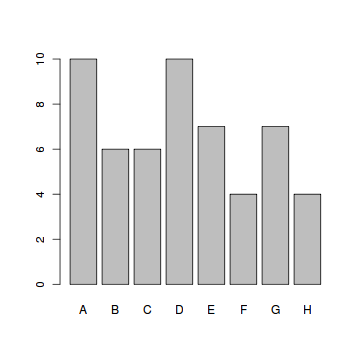
\includegraphics[height=0.3\textheight]{art/categorical-data1x}
\caption[Bar Plot]{The Bar-Plot. \newline
\url{http://www.r-tutor.com/elementary-statistics/qualitative-data/bar-graph}}
\label{fig:barplot}
\end{figure}



\subsubsection{Bivariate}
Visualizing a two-way cross-table can be done using an extension of the bar-plot.
Several extensions exist. By far, the most informative and recommended figure, in this author's view, is the \emph{mosaic plot}, illustrated in Figure~\ref{fig:mosaic}. \marginnote{Mosaic Plot}

\begin{figure}[h]
\centering
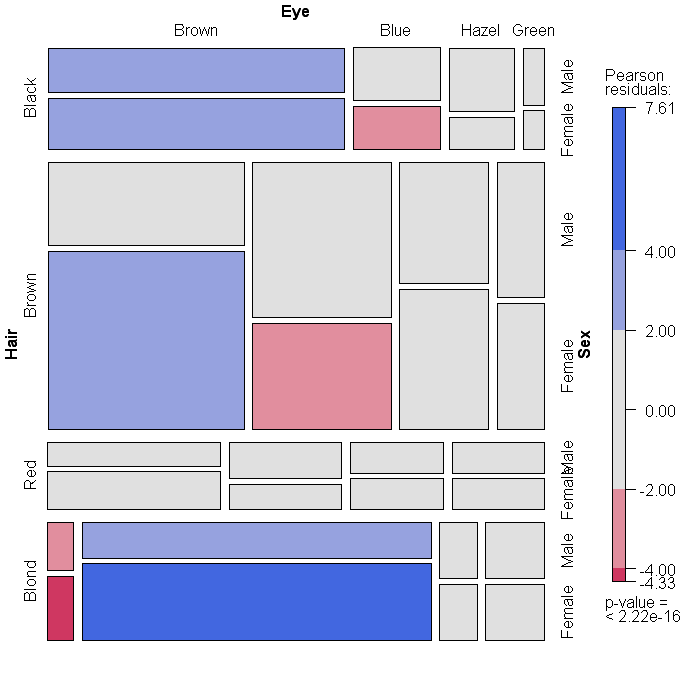
\includegraphics[height=0.3\textheight]{art/mosaic1}
\caption[Mosaic Plot]{Mosaic Plot. \newline
\url{http://www.statmethods.net/advgraphs/mosaic.html}}
\label{fig:mosaic}
\end{figure}







\afterpage{\clearpage}


\subsection{Visualizing Continuous Data}




\subsubsection{Univariate}
Visualization of univariate continuous vectors can present the raw data, or it distribution (i.e.- discarding the indexes).
The most basic visualizations are the \emph{dotchart}, \emph{histogram}, \emph{boxplot}, \emph{stem-and-leaf plot}. 
These are illustrated in figures \ref{fig:dot_plot}, \ref{fig:histogram_eruptions}, \ref{fig:boxplot}, \ref{fig:stem_and_leaf} respectively. 
[TODO: add QQplot and QQnorm]

 
\begin{figure}[h]
\centering
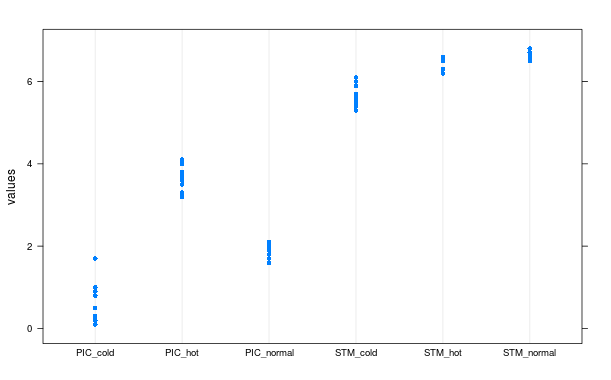
\includegraphics[height=0.3\textheight]{art/lmCm0}
\caption[Dot Plot]{Dot Plot. \newline \url{http://stackoverflow.com/questions/15109822/r-creating-scatter-plot-from-data-frame}}
\label{fig:dot_plot}
\end{figure}



\begin{figure}[h]
\centering
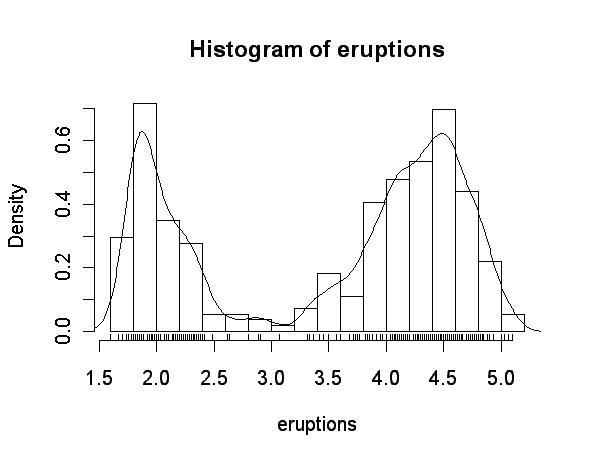
\includegraphics[height=0.3\textheight]{art/histogram_eruptions}
\caption[Histogram]{Histogram. \newline
\url{http://compbio.pbworks.com/w/page/16252882/Basic}}
\label{fig:histogram_eruptions}
\end{figure}

\begin{figure}[h]
\centering
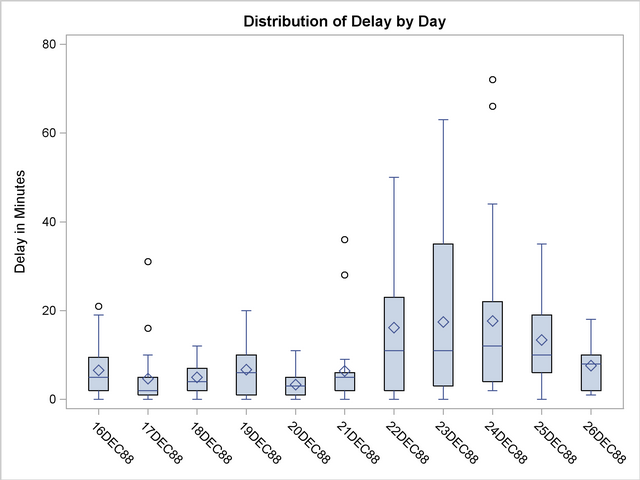
\includegraphics[height=0.3\textheight]{art/ex6aout}
\caption[BoxPlot]{Boxplot. \newline \url{http://support.sas.com/documentation/cdl/en/statug/63033/HTML/default/viewer.htm}}
\label{fig:boxplot}
\end{figure}



\begin{figure}[h]
\centering
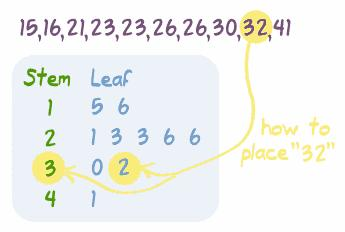
\includegraphics[height=0.3\textheight]{art/stem_and_leaf}
\caption[Stem and Leaf Pot]{Stem-and-leaf plot. \newline
\url{https://www.mathsisfun.com/data/stem-leaf-plots.html}}
\label{fig:stem_and_leaf}
\end{figure}




\subsubsection{Bivariate}
The simultaneous visualization of two continuous variables, can naturally be done with a \emph{scatter plot}.
More sophisticated visualization, which generalizes the histogram into two dimensions, is the \emph{hexbin plot}.  
These are illustrated in figures \ref{fig:scatterplot}, and \ref{fig:hexbin}, respectively. 


\begin{figure}[h]
\centering
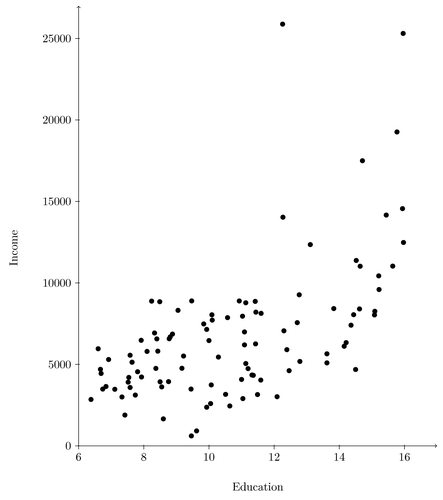
\includegraphics[height=0.3\textheight]{art/scatterplot}
\caption[Scatter Plot]{Scatter Plot. \newline 
\url{http://texample.net/tikz/examples/scatterplot/}}
\label{fig:scatterplot}
\end{figure}





\begin{figure}[h]
\centering
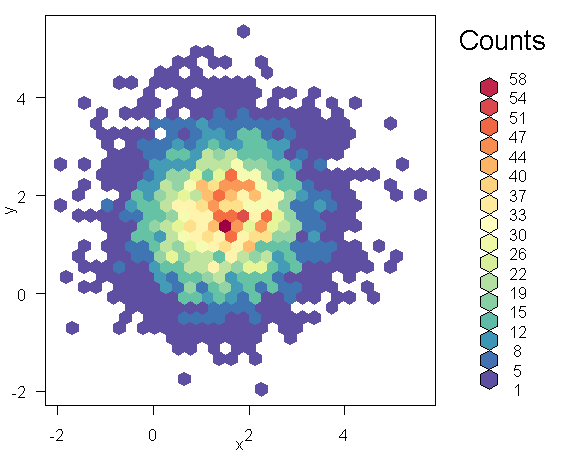
\includegraphics[height=0.3\textheight]{art/hexbin2}
\caption[HexBin Plot]{HexBin plot. Sorce: \url{http://www.r-bloggers.com/5-ways-to-do-2d-histograms-in-r/}}
\label{fig:hexbin}
\end{figure}






\subsubsection{Multivariate Data}
Since we cannot possibly visualize data in more than $3$-dimensions, and we clearly prefer data in $1$ or $2$ dimensions, the visualization of multivariate data will typically consist of summarizing the data into $1D$ or $2D$, and then applying the above mentioned visualization techniques.

An important exception is due to the observation that a computer image, is essentially a matrix. 
We can thus visualize matrices, with a simple image, and in particular, covariance and correlation matrices, as illustrated in Figure~\ref{fig:covariance_image}.

A second exception is when the data has both continous variables and discrete attributes. 
Endlessly many combinations are then possible.
The author strongly recommends to visit Hans Rosling's \emph{Gap Minder} at \url{http://www.gapminder.org/world} for an excellent interactive visualization. \marginnote{Gap Minder}


\begin{figure}[h]
\centering
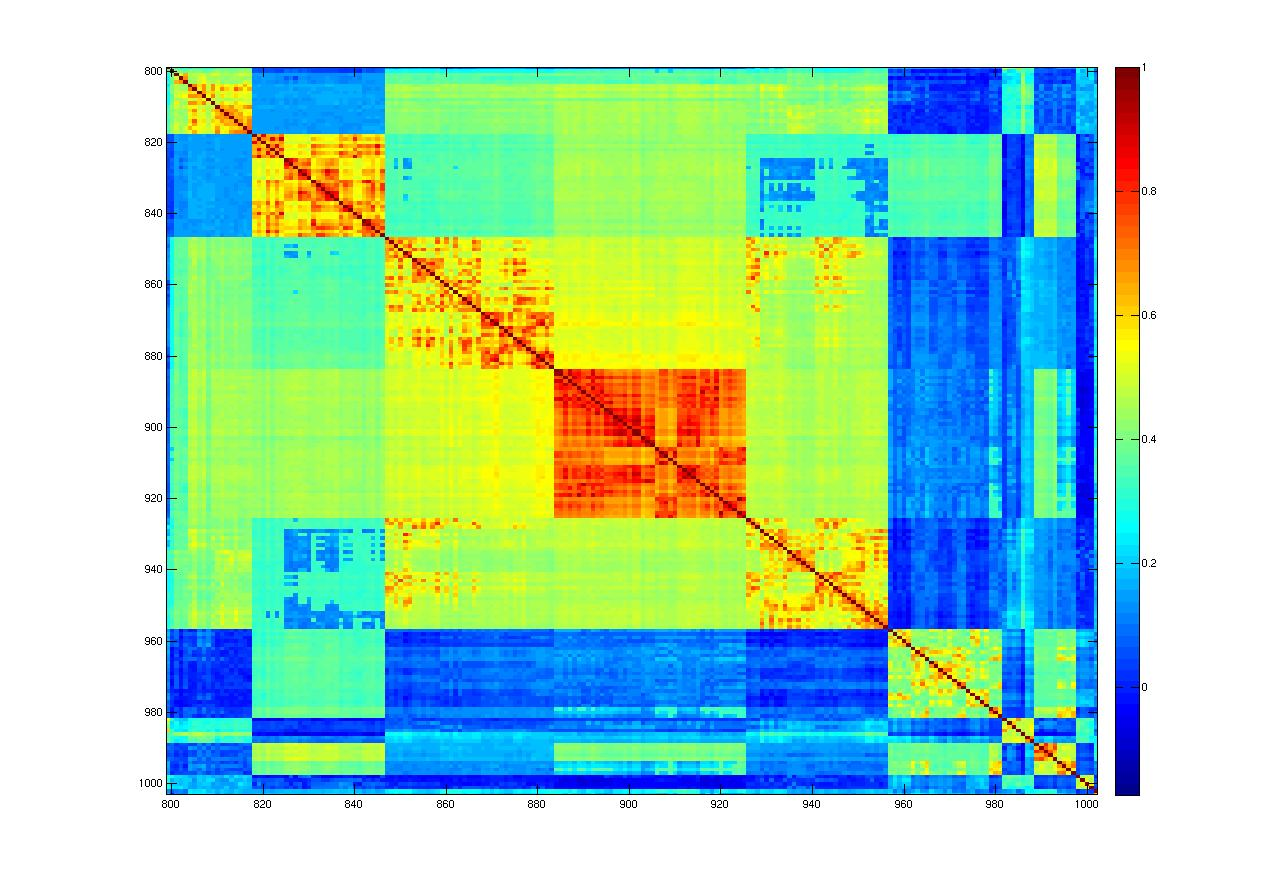
\includegraphics[height=0.3\textheight]{art/covarianceSupervised}
\caption[Covariance Matrix]{Image of covariance matrix. \newline
\url{http://cs.brown.edu/courses/csci1950-g/results/final/sghosh/}}
\label{fig:covariance_image}
\end{figure}




\subsection{On-Line Visualization}
For the purpose of quality control, we may often want an \emph{on-line} visualization, and not \emph{off-line}, as the ones previously discussed.
This is the purpose of \emph{dashboards}, illustrated in Figure~\ref{fig:dashboard}.\marginnote{Dashboard}

\begin{figure}[h]
\centering
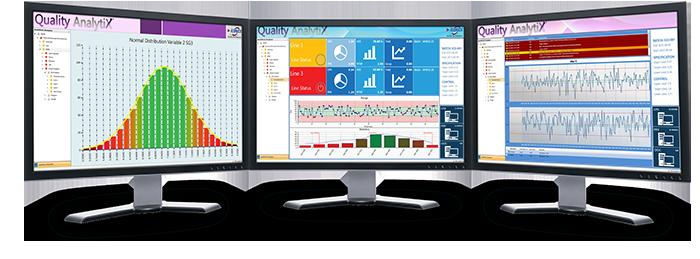
\includegraphics[height=0.3\textheight, width=0.9\linewidth]{art/dashboard}
\caption[Dashboard]{Dashboard. \newline
\url{http://www.iconics.com/Home/Products/AnalytiX/Quality-AnalytiX.aspx}}
\label{fig:dashboard}
\end{figure}

\afterpage{\clearpage}
